% Options for packages loaded elsewhere
\PassOptionsToPackage{unicode}{hyperref}
\PassOptionsToPackage{hyphens}{url}
\documentclass[
]{article}
\usepackage{xcolor}
\usepackage{amsmath,amssymb}
\setcounter{secnumdepth}{-\maxdimen} % remove section numbering
\usepackage{iftex}
\ifPDFTeX
  \usepackage[T1]{fontenc}
  \usepackage[utf8]{inputenc}
  \usepackage{textcomp} % provide euro and other symbols
\else % if luatex or xetex
  \usepackage{unicode-math} % this also loads fontspec
  \defaultfontfeatures{Scale=MatchLowercase}
  \defaultfontfeatures[\rmfamily]{Ligatures=TeX,Scale=1}
\fi
\usepackage{lmodern}
\ifPDFTeX\else
  % xetex/luatex font selection
\fi
% Use upquote if available, for straight quotes in verbatim environments
\IfFileExists{upquote.sty}{\usepackage{upquote}}{}
\IfFileExists{microtype.sty}{% use microtype if available
  \usepackage[]{microtype}
  \UseMicrotypeSet[protrusion]{basicmath} % disable protrusion for tt fonts
}{}
\makeatletter
\@ifundefined{KOMAClassName}{% if non-KOMA class
  \IfFileExists{parskip.sty}{%
    \usepackage{parskip}
  }{% else
    \setlength{\parindent}{0pt}
    \setlength{\parskip}{6pt plus 2pt minus 1pt}}
}{% if KOMA class
  \KOMAoptions{parskip=half}}
\makeatother
\usepackage{longtable,booktabs,array}
\usepackage{calc} % for calculating minipage widths
% Correct order of tables after \paragraph or \subparagraph
\usepackage{etoolbox}
\makeatletter
\patchcmd\longtable{\par}{\if@noskipsec\mbox{}\fi\par}{}{}
\makeatother
% Allow footnotes in longtable head/foot
\IfFileExists{footnotehyper.sty}{\usepackage{footnotehyper}}{\usepackage{footnote}}
\makesavenoteenv{longtable}
\usepackage{graphicx}
\makeatletter
\newsavebox\pandoc@box
\newcommand*\pandocbounded[1]{% scales image to fit in text height/width
  \sbox\pandoc@box{#1}%
  \Gscale@div\@tempa{\textheight}{\dimexpr\ht\pandoc@box+\dp\pandoc@box\relax}%
  \Gscale@div\@tempb{\linewidth}{\wd\pandoc@box}%
  \ifdim\@tempb\p@<\@tempa\p@\let\@tempa\@tempb\fi% select the smaller of both
  \ifdim\@tempa\p@<\p@\scalebox{\@tempa}{\usebox\pandoc@box}%
  \else\usebox{\pandoc@box}%
  \fi%
}
% Set default figure placement to htbp
\def\fps@figure{htbp}
\makeatother
\setlength{\emergencystretch}{3em} % prevent overfull lines
\providecommand{\tightlist}{%
  \setlength{\itemsep}{0pt}\setlength{\parskip}{0pt}}
\usepackage{bookmark}
\IfFileExists{xurl.sty}{\usepackage{xurl}}{} % add URL line breaks if available
\urlstyle{same}
\hypersetup{
  pdftitle={OmniScale Gravity --- 1-Page TEASER (v4.6)},
  pdfauthor={Christian (Cruz) deWilde and ChatGPT-5 (Thinking \& Pro)},
  hidelinks,
  pdfcreator={LaTeX via pandoc}}

\title{OmniScale Gravity --- 1-Page TEASER (v4.6)}
\author{\protect\phantomsection\label{_Hlk206169066}{}Christian (Cruz)
deWilde and ChatGPT-5 (Thinking \& Pro)}
\date{2025-08-15}

\begin{document}
\maketitle

~

\section{One potential, conservative
scope}\label{one-potential-conservative-scope}

Identify \(\Phi \equiv c^{2}\chi\) and use the weak-field/1PN metric
with \(\beta = \gamma = 1\) as a bookkeeping device on a flat
background. Use the same \(\Phi\) for light \emph{and} motion; GW sector
is conservative (\(v = c\), \(+ / \times\) only; no scalar dipole).
Low-\(g\) closure A/B keeps the field scalar and curl-free in general.

\section{STATUS OF SECTORS (mini)}\label{status-of-sectors-mini}

\begin{longtable}[]{@{}
  >{\raggedright\arraybackslash}p{(\linewidth - 4\tabcolsep) * \real{0.2467}}
  >{\raggedright\arraybackslash}p{(\linewidth - 4\tabcolsep) * \real{0.3861}}
  >{\raggedright\arraybackslash}p{(\linewidth - 4\tabcolsep) * \real{0.3672}}@{}}
\toprule\noalign{}
\begin{minipage}[b]{\linewidth}\raggedright
\textbf{Sector}
\end{minipage} & \begin{minipage}[b]{\linewidth}\raggedright
\textbf{Now}
\end{minipage} & \begin{minipage}[b]{\linewidth}\raggedright
\textbf{Next}
\end{minipage} \\
\midrule\noalign{}
\endhead
\bottomrule\noalign{}
\endlastfoot
\(\chi\) \& \(\Phi\) & Map \(\Phi = c^{2}\chi\); closure A/B & Derive
from action \\
Metric \(1\)PN & \(\beta = \gamma = 1\) & Derive including \(g_{0i}\) \\
\(g_{0i}\) & Assume GR \(( - 4V_{i}/c^{3})\) & Predict
Lense--Thirring \\
GWs & \(v = c\), \(+ / \times\) only & Maintain pulsar/GW safety \\
\end{longtable}

\section{Decisive falsifiers}\label{decisive-falsifiers}

Frame dragging; PPN \(\gamma,\beta\); \(v_{gw} \neq c\) or extra GW
polarizations; no LOS-environment correlation of \(H_{0}\) after
systematics.

\section{Why it matters}\label{why-it-matters}

One shared \(\Phi\) ties orbits, lensing, and time delays; fewer knobs
\(\Rightarrow\) stronger tests.

\section{FIGURES}\label{figures}

\begin{longtable}[]{@{}
  >{\raggedright\arraybackslash}p{(\linewidth - 4\tabcolsep) * \real{0.3340}}
  >{\raggedright\arraybackslash}p{(\linewidth - 4\tabcolsep) * \real{0.3340}}
  >{\raggedright\arraybackslash}p{(\linewidth - 4\tabcolsep) * \real{0.3321}}@{}}
\toprule\noalign{}
\begin{minipage}[b]{\linewidth}\centering
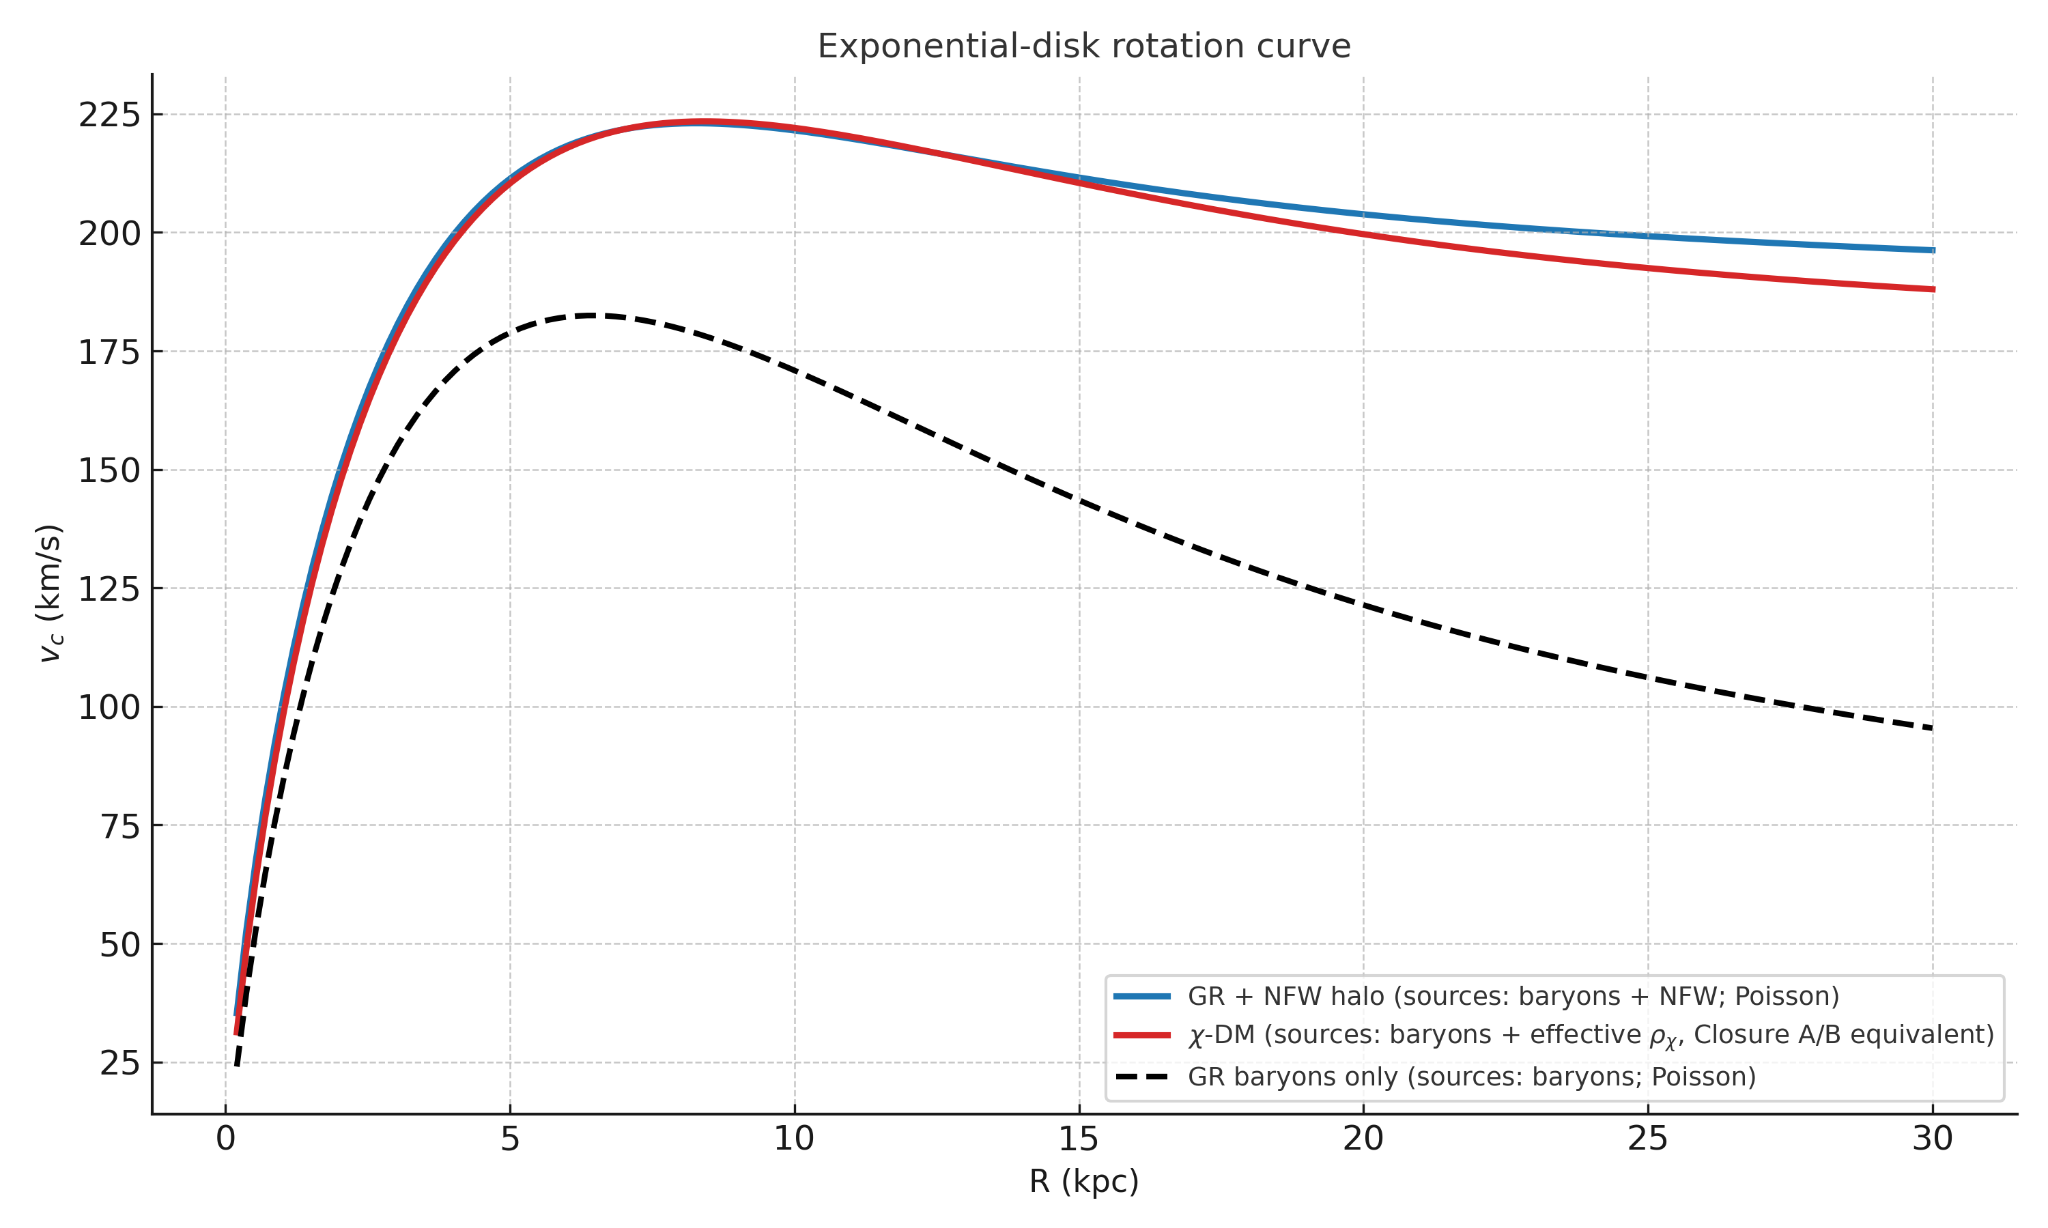
\includegraphics[width=2.10832in,height=1.26417in,alt={image}]{teaser_media/media/image1.png}\emph{RC:}
\(\mathbf{v}_{\mathbf{c}}\) (km/s) vs \(\mathbf{R}\) (kpc).
\end{minipage} & \begin{minipage}[b]{\linewidth}\centering
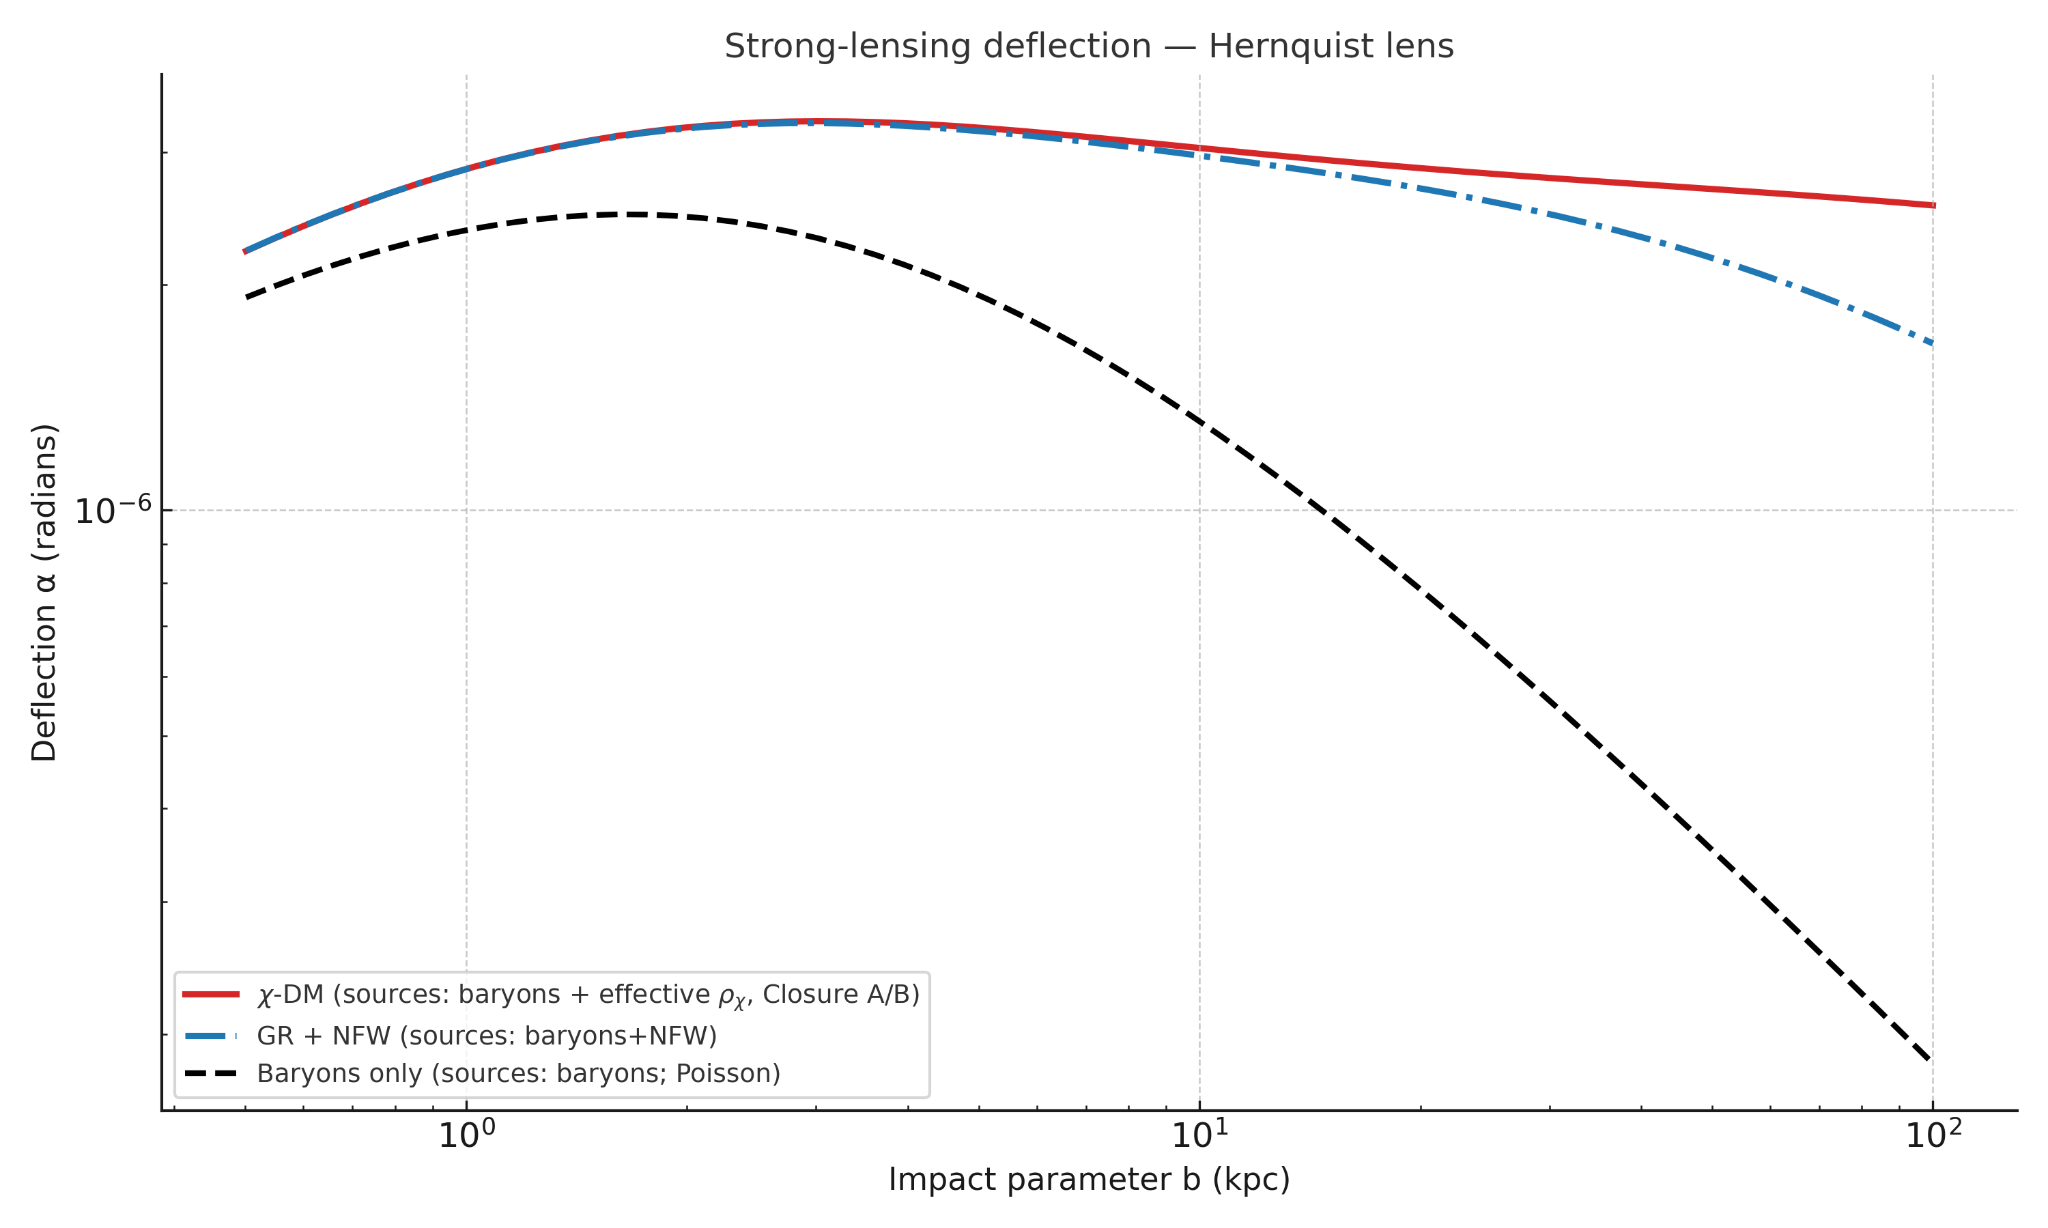
\includegraphics[width=2.10189in,height=1.26031in,alt={image}]{teaser_media/media/image2.png}Deflection:
\(\mathbf{\alpha}\mathbf{(}\mathbf{b}\mathbf{)}\) (radians).
\end{minipage} & \begin{minipage}[b]{\linewidth}\centering
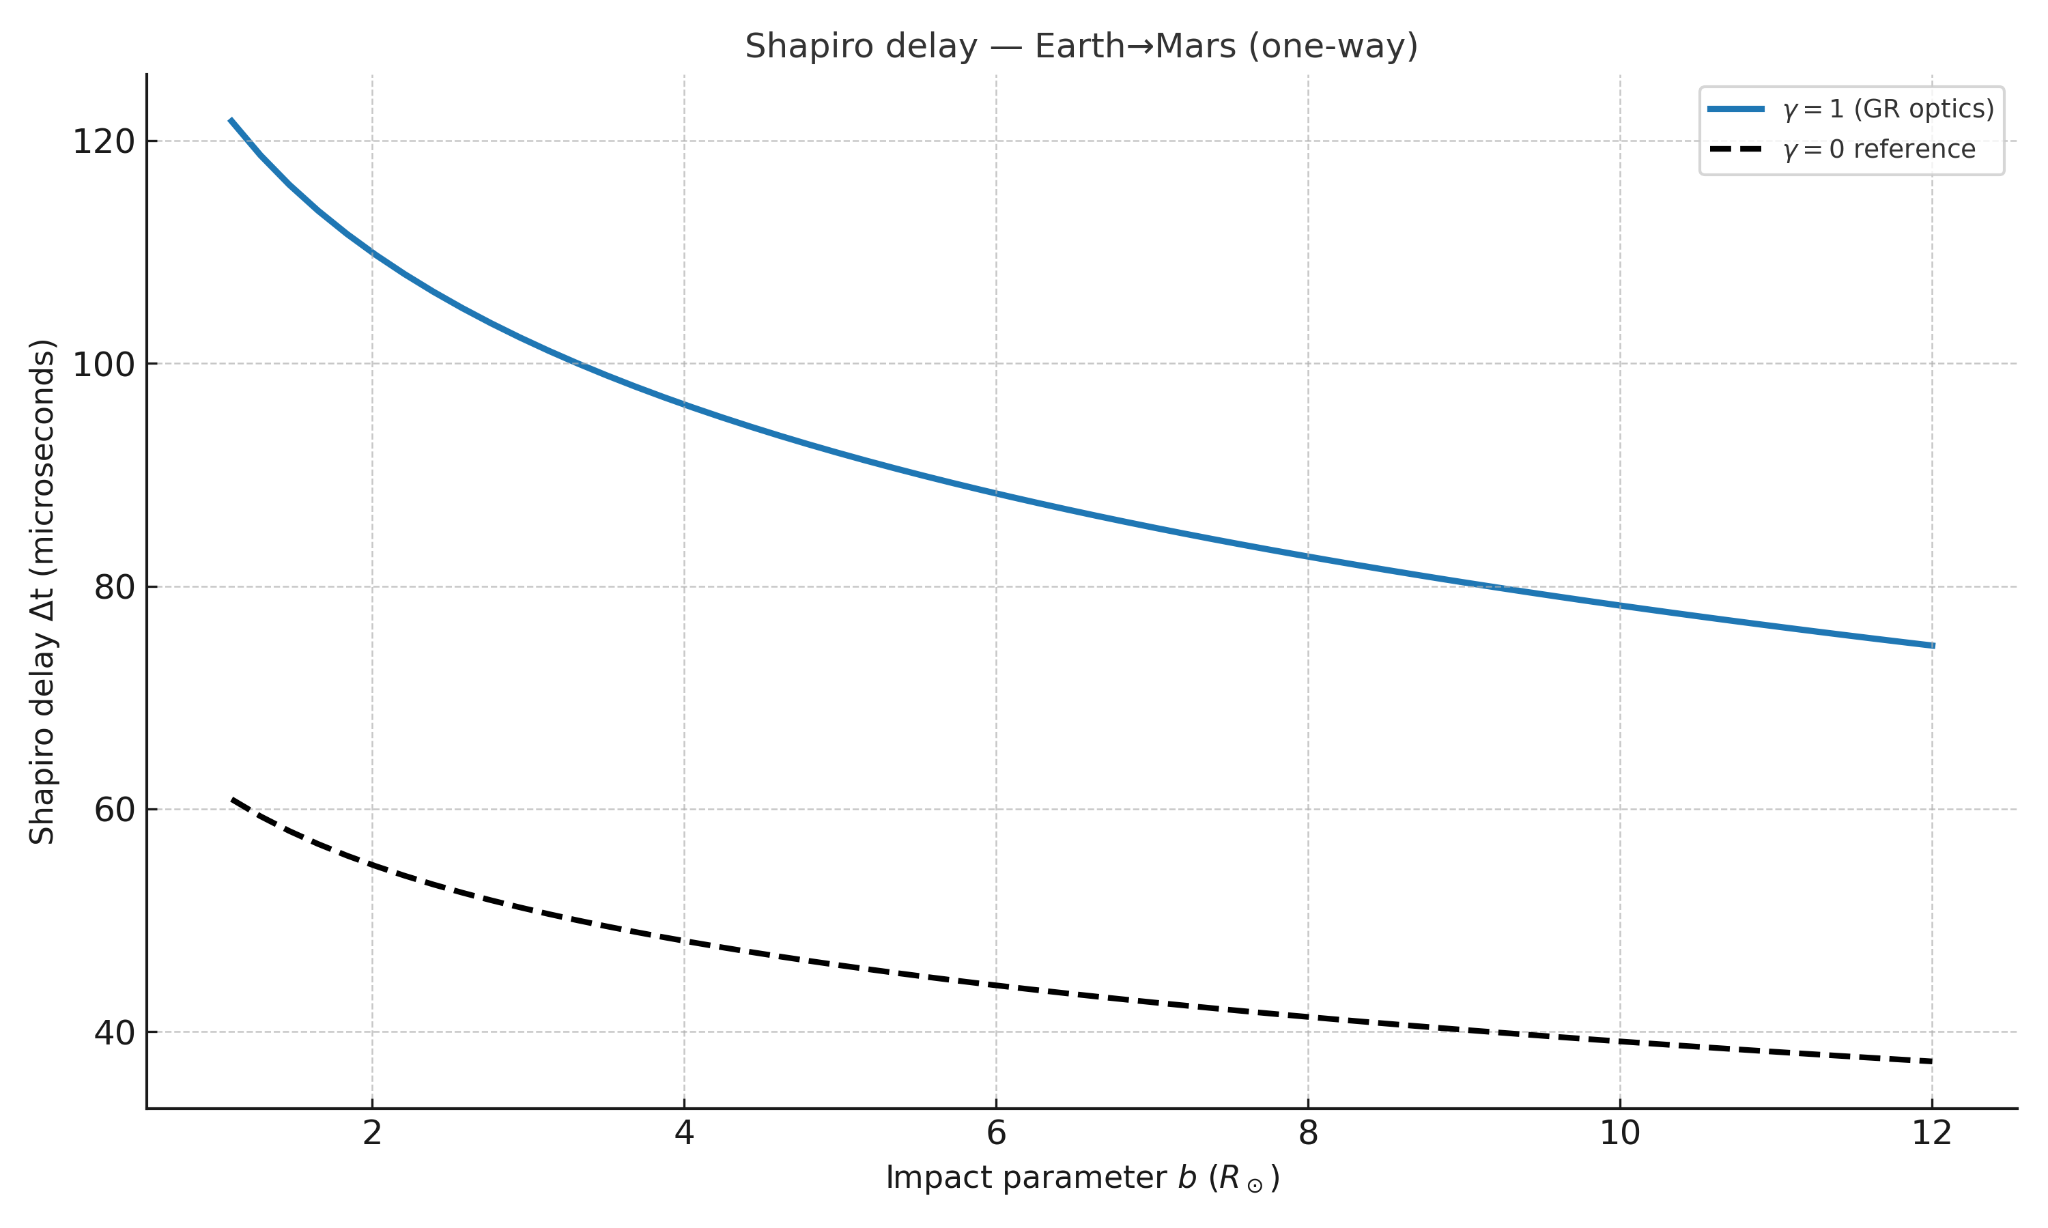
\includegraphics[width=2.0885in,height=1.25228in,alt={image}]{teaser_media/media/image3.png}\emph{Shapiro:}
\(\mathbf{\Delta}\mathbf{t}\) (µs) vs
\(\mathbf{b}\mathbf{/}\mathbf{R}_{\mathbf{\odot}}\).
\end{minipage} \\
\midrule\noalign{}
\endhead
\bottomrule\noalign{}
\endlastfoot
\end{longtable}

\end{document}
